\documentclass[tikz]{standalone}
\usepackage{pgfplots}
\pgfplotsset{compat=1.15}
\usepackage{mathrsfs}
\usetikzlibrary{arrows,calc}
\usepackage{tkz-euclide}
\pagestyle{empty}

\definecolor{AngleClr}{rgb}{0,0.39215686274509803,0}
\definecolor{ShapeClr}{rgb}{0.6,0.2,0}

\begin{document}

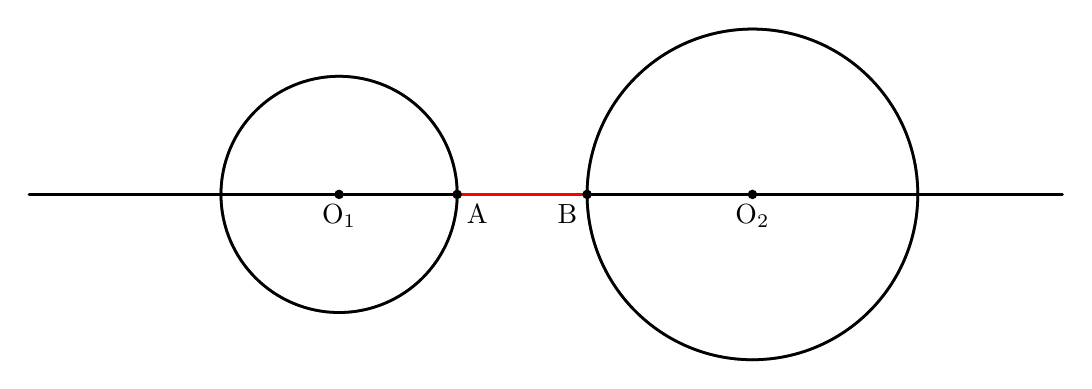
\begin{tikzpicture}[scale=.75]
\tkzSetUpLine[line width=1pt,color=black]
\tkzSetUpPoint[fill=black]

\tkzDefPoints{0/0/O1,7/0/O2,2/0/A,4.2/0/B}


\tkzDrawCircle[line width=1.0pt,fill=white](O1,A)
\tkzDrawCircle[line width=1.0pt,fill=white](O2,B)

\tkzDrawSegments[line width=1pt,color=black,add=0.75 and 0.75](O1,O2)
\tkzDrawSegments[line width=1pt,color=red](A,B)

\tkzDrawCircle[line width=1.0pt,color=black](O1,A)
\tkzDrawCircle[line width=1.0pt,color=black](O2,B)


\tkzDrawPoints[size=3](O1,O2,A,B)
\tkzLabelPoint[below](O1){$\rm O_1$}
\tkzLabelPoint[below](O2){$\rm O_2$}
\tkzLabelPoint[below right](A){$\rm A$}
\tkzLabelPoint[below left](B){$\rm B$}

\end{tikzpicture}
\end{document}
